\documentclass[a4j,11pt]{jarticle}
\usepackage{fancyheadings}
\usepackage{here}
\usepackage[dvipdfmx]{graphicx}
\renewcommand{\thepage}{\small -- \arabic{page} --}
%\headrulewidth=0pt
\rhead{}
\lhead{}
\textheight 234mm
%
\usepackage{amsmath,amssymb}
\usepackage{bm}
\usepackage{ascmac}
\usepackage{color}
\usepackage{listings,jvlisting}
\usepackage{enumerate}
\usepackage{url}
\newcommand{\thisyear}{1}
\pagestyle{fancy}
\lhead{{\number\year}年度 信号処理特論1}
\title{{\number\year}年度 信号処理特論1}
\date{\number\year 年\number\month 月\number\day 日}
\author{36414067  飯田 諒 \\ メディア情報プログラム\\徳田・南角・橋本研究室}
%
%
\lstset{
    language=Python,
    commentstyle=\color{gray}\ttfamily,
    basicstyle={\ttfamily},
    identifierstyle={\small},
    commentstyle={\smallitshape},
    keywordstyle={\small\bfseries},
    ndkeywordstyle={\small},
    stringstyle={\small\ttfamily},
    frame={tb},
    breaklines=true,
    columns=[l]{fullflexible},
    numbers=left,
    xrightmargin=0zw,
    xleftmargin=3zw,
    numberstyle={\scriptsize},
    stepnumber=1,
    numbersep=1zw,
    lineskip=-0.5ex
}
\begin{document}
    \maketitle
    \thispagestyle{empty}
    \clearpage
    
    \begin{itemize}
        \item 使用した音:自分自身の声
        \item 使用したソフト:WaveSufer
        \item 使用した機材:自身の計算機
        \item 使用したOS:Windows
        \item プログラミング言語:Python
    \end{itemize}
    課題のソースコードの詳細は資料の最後尾にまとめて載せる。
    \section{課題1}
    まず、フーリエ級数展開の式は以下のとおりである。\\
    $$A_n = \frac 2 T \int _{-\frac T 2} ^{\frac T 2} f(x) \cos{\left( \frac {2\pi} T n x \right)} dx$$
    $$B_n = \frac 2 T \int _{-\frac T 2} ^{\frac T 2} f(x) \sin{\left( \frac {2\pi} T n x \right)} dx$$
    この式を、離散データに対して使うために変換する。主に$A_n$について考える。\\
    この式の意味は、正規直交基底を満たす、$\frac 2 T \cos{ \left( \frac {2\pi} T n x \right)} (-\frac T 2 \leq x \leq \frac T 2), (n = 1, 2, 3, ...)$と、
    関数$f(x)$との内積を取って、$f(x)$の成分分解をしている。(係数である$\frac 2 T$は、$\left< \cos{ \left( \frac {2\pi} T n x \right)},\cos{\left( \frac {2\pi} T n x \right)} \right> 
    = \int _{-\frac T 2} ^{\frac T 2} \cos{ ^2 \left( \frac {2\pi} T n x \right) } dx = \frac T 2$であるため、正規性を保つために割っている。)
    また、$\frac 2 T \cos{\left( \frac {2\pi} T n x \right)}$は、$-\frac T 2 \leq x \leq \frac T 2$の間で、$n$回振動しているから、$n[Hz]$の信号である。
    これらの理由で、フーリエ級数展開は$0 \sim n[Hz]$までの成分を分解している。この原理を利用して、今回の離散信号に対して$A_n$を求める。\\
    $\cos{ \left( \frac {2\pi} {Fs} x \right)}$は、$0 \leq x \leq Fs$で、$1[Hz]$であるから、$f[Hz]$は$\cos{ \left( \frac {2\pi} {Fs} f x \right)}$である。
    また、$x$は整数値しか取れないため、 積分を考えるとき区分求積法を考える。区分求積法の式は以下のとおりである。
    $$\int _b ^a f(x) dx = \lim _{n \to \infty} \frac 1 n \sum _{k = bn} ^{an-1} f\left(\frac k n\right)$$
    xが整数のみを考えたいため、$n = 1$とすると、
    $$\int _b ^a f(x) dx = \sum _{k = bn} ^{an-1} f(k)$$
    となる。そして、$T[s]$で周期性があると考えると、$N = Fs \cdot T$点で周期を持っている。
    これらの考え方から、$A(f)$を定義すると、
    \begin{align}
        A(f) &= \int _0 ^N f(x) \frac {\cos{ \left( \frac {2\pi} {Fs} f x \right)}} {\left< \cos{ \left( \frac {2\pi} {Fs} f x \right)}, \cos{ \left( \frac {2\pi} {Fs} f x \right)} \right>} dx \\
        &= \frac 1 {\left< \cos{ \left( \frac {2\pi} {Fs} f x \right)}, \cos{ \left( \frac {2\pi} {Fs} f x \right)} \right>} \int _0 ^N f(x) \cos{ \left( \frac {2\pi} {Fs} f x \right)}  dx\\
        &\approx \frac 1 {\left< \cos{ \left( \frac {2\pi} {Fs} f x \right)}, \cos{ \left( \frac {2\pi} {Fs} f x \right)} \right>} \sum _{k = 0} ^{ N -1 } f(k) \cos{ \left( \frac {2\pi} {Fs} f k \right)}
    \end{align}
    この時、$\left< \cos{ \left( \frac {2\pi} {Fs} f x \right)}, \cos{ \left( \frac {2\pi} {Fs} f x \right)} \right>$を計算すると、
    \begin{align}
        \left< \cos{ \left( \frac {2\pi} {Fs} f x \right)}, \cos{ \left( \frac {2\pi} {Fs} f x \right)} \right>
        &= \int _0 ^N \cos{ ^2 \left( \frac {2\pi} {Fs} f x \right)} dx\\
        &= \cdots\\
        &= \frac 1 2 (N + \frac {Fs} {4\pi f N}sin(\frac {4\pi} {Fs} f N ))\\
        &\approx \frac 2 N
    \end{align}
    最後の近似は、$\left| \frac {\sin x} x \right| \leq 1 \ll N$を用いた。
    以上より、$B_n$も同様の議論をすると、
    $$A(f) =  \frac N 2 \sum _{k = 0} ^{ N -1 } f(k) \cos{ \left( \frac {2\pi} {Fs} f k \right)}$$
    $$B(f) =  \frac N 2 \sum _{k = 0} ^{ N -1 } f(k) \sin{ \left( \frac {2\pi} {Fs} f k \right)}$$
    この時、$f$は連続値を取ってよいが、今回求めたい$H_n(nは整数)$は、$n[Hz]$の周波数の係数を表すため、
    $H_n = \sqrt{A_n ^2 + B_n^2} = \sqrt{A(n) ^2 + B(n)^2}$である。\\
    本問題では$H_n$を求めるという問題であるが、連続値にできるため線グラフで表す。\\

    サンプリング周波数はFs = 16000とした。\\
    Nをどんな値にするかに関して、Nが大きくなると高い周波数分解能が得られるが、時間分解能(より局所的な時間を見る能力)が減り、
    逆にNを小さくすると周波数分解能が低くなり時間分解能が高くなる。したがって、これら二つの能力はトレードオフの関係にある。
    今回は、倍音について深く考察したいと考えたため、Nを大きくし周波数分解能を高くした。具体的にはN=1024にした。

    プログラムについて述べる。最初に音声データの最大値を取り、時系列すべてに対して割ることで正規化をする。
    次に、適当に音声が出ているところを選び、N点とるために、全データ区間から、start\_iter \~ start\_iter +Nを切り出す。
    次に、ブラックマン窓を掛ける。
    次に、A(f)を求めるため、Af[]という配列を作り、for文で足し合わせ、最後に$\frac 2 N$を掛けた。
    また今回はfを滑らかに描画したいと考えたため、fを計算する間隔をdelta\_fという変数で定めた。
    しかし、delta\_fが0.5の時はA[0.5],A[3.5]といった配列は用意できないため、$Af[1] = A(0.5), Af[2] = A(1), Af[3] = A(1.5)$つまり、
    $Af[f] = A(f\cdot delta\_f)$と定めた。
    最後にHnを計算して描画するという流れである。
    ここでは主要なコードのみ載せる。
    \begin{lstlisting}[language = Python , caption = fourier.py]
data_from_window = np.zeros(len(norm_data))
for i in range(N) :
    data_from_window[i] = norm_data[i+start_iter]*brackman_window(i,N)

Af = np.zeros(int(max_f/delta_f + 1))
Bf = np.zeros(int(max_f/delta_f + 1))

for f in range(len(Af)) :
    for j in range(N) :
        Af[f] += data_from_window[j] * math.cos(2*math.pi/Fs*f*delta_f*j)
        Bf[f] += data_from_window[j] * math.sin(2*math.pi/Fs*f*delta_f*j)
    Af[f] *= 2/N
    Bf[f] *= 2/N
    \end{lstlisting}
    入力音声波形、フーリエ級数展開のグラフは図\ref{fig:input}、図\ref{fig:fourier}のとおりである。
    \begin{figure}[tb]
        \centering
        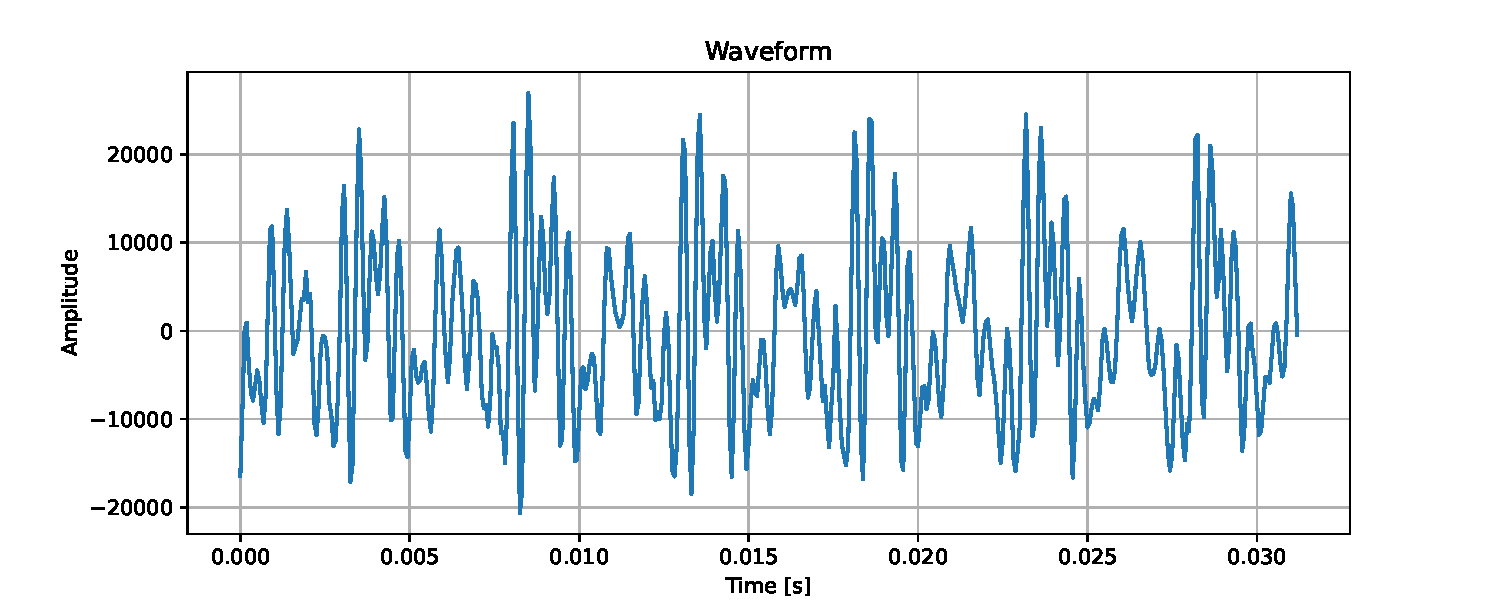
\includegraphics[width=0.8\hsize]{../../figure/arayurugennzituwo.pdf}
        \caption{入力音声波形}
        \label{fig:input}
    \end{figure}
    \begin{figure}[tb]
        \centering
        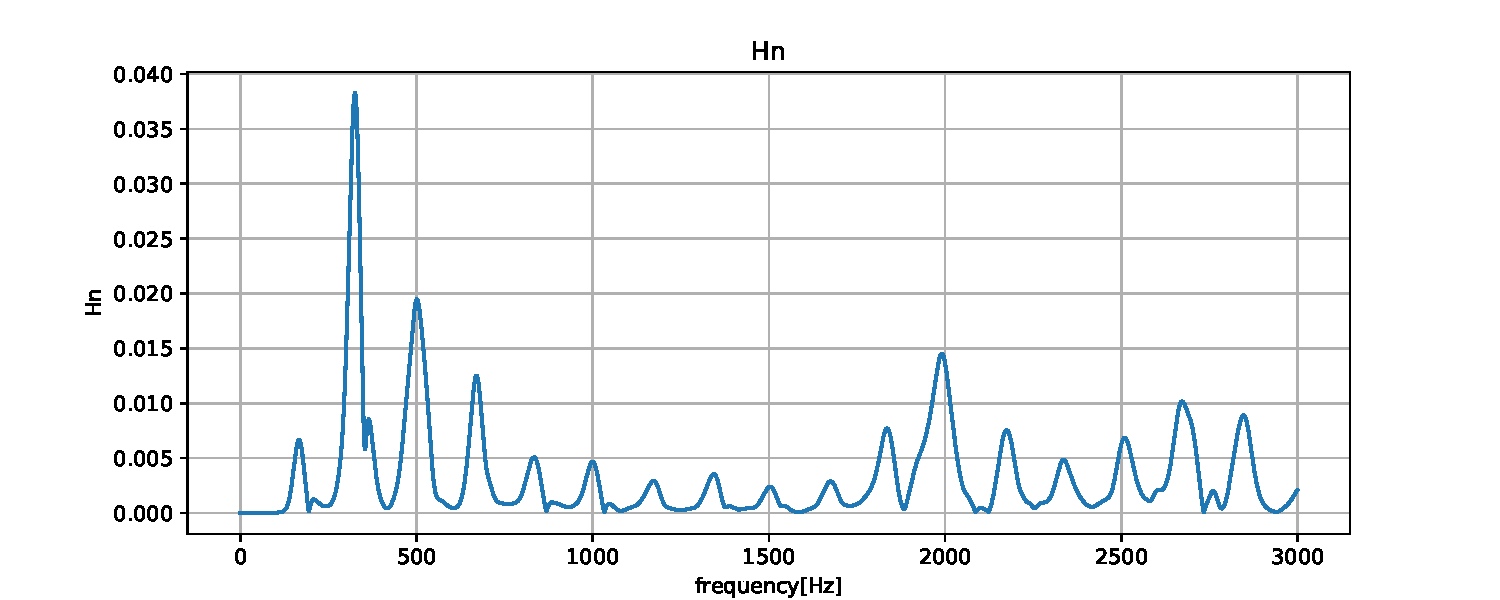
\includegraphics[width=0.8\hsize]{../../figure/arayurugennzituwo_Hn.pdf}
        \caption{フーリエ級数展開グラフ,N = 1024,Fs = 16000,delta\_f = 0.5}
        \label{fig:fourier}
    \end{figure}
    これを観察すると、167[Hz]程にフォルマントがあり、倍音として167の整数倍のところにもフォルマントがあることが分かる。
    \section{課題2}
    LPFに通した音声波形、フィルタに通した後のフーリエ級数展開のグラフは図\ref{fig:LPF}、図\ref{fig:LPF_fourier}のとおりである。
    \begin{figure}[tb]
        \centering
        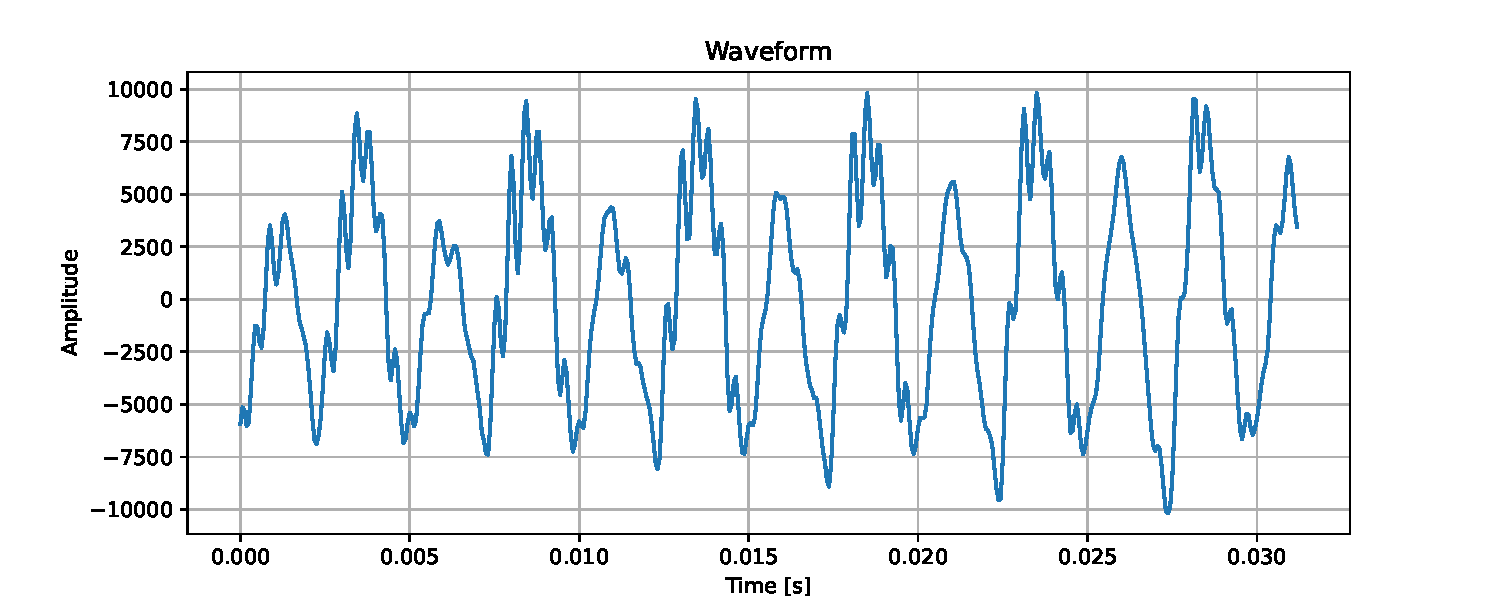
\includegraphics[width=0.8\hsize]{../../figure/arayurugennzituwo_LPF_reconst.pdf}
        \caption{LPF通過後音声波形}
        \label{fig:LPF}
    \end{figure}
    \begin{figure}[tb]
        \centering
        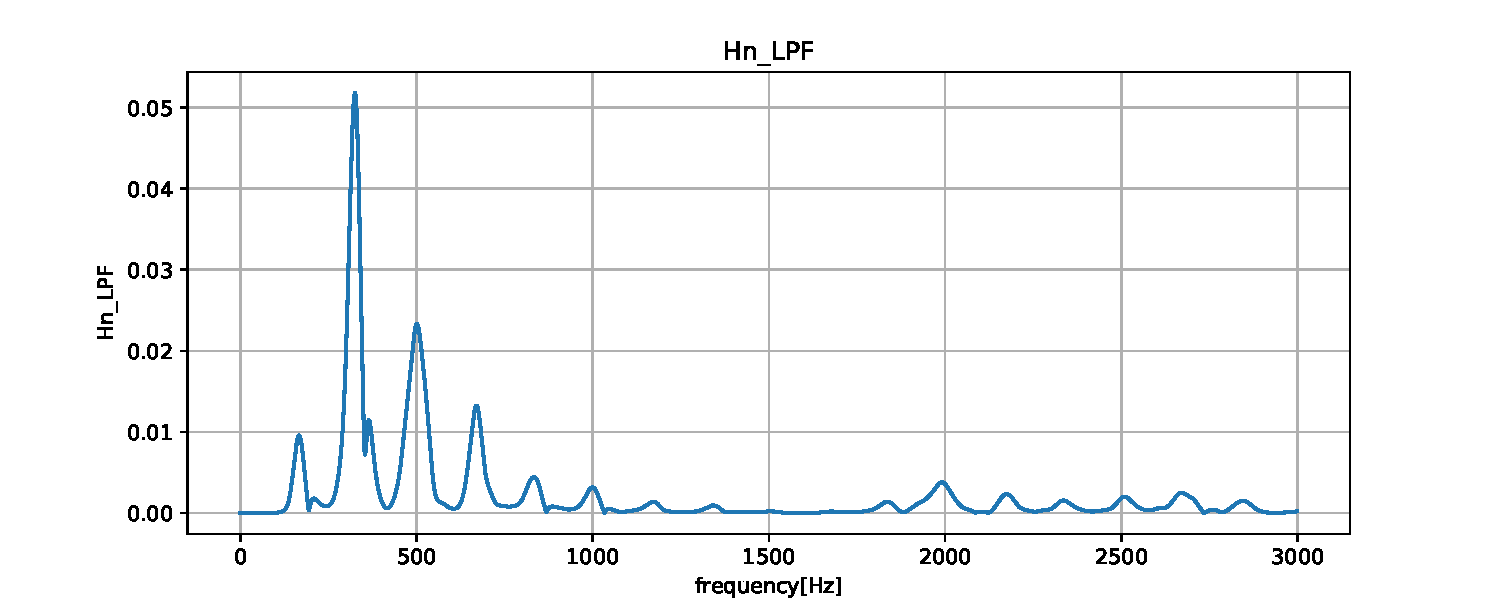
\includegraphics[width=0.8\hsize]{../../figure/arayurugennzituwo_Hn_LPF.pdf}
        \caption{LPF通過後フーリエ級数展開グラフ,N = 1024,Fs = 16000 , delta\_f = 0.5}
        \label{fig:LPF_fourier}
    \end{figure}
    まず図\ref{fig:input}と図\ref{fig:LPF}の音声波形を観察する。
    LPFの関数は時間方向に幅を持った10点に関する平均を取っている(時間移動平均)ため、高周波成分に対して鈍感にする性能を持っているフィルタであり、
    LPFという名の通り、低周波成分を通すフィルタである。
    図を見比べると、確かに細かな振動、つまり高周波成分がなくなり、荒い波の信号になっていることが読み取れる。

    また図\ref{fig:fourier}と図\ref{fig:LPF_fourier}を見比べると、これも高周波成分である
    1000[Hz]以降からフォルマントが小さくなっていることが読み取れる。
    また逆に低周波成分では振幅スペクトルが大きくなっていることも読み取れる。これは高周波成分の移動平均が
    倍音成分と一致する要素があるため、その分大きくなっていると考察する。
    \section{課題3}
    試聴した感想は、LPFを通した後では、音がこもったように聞こえた。これは高周波成分が聞こえなくなったことによって
    相対的に低周波成分、つまりこもった音の成分が際立って聞こえたためであると考察した。
    \section{ソースコードの主要部}
    \subsection{課題1}
    \begin{lstlisting}[language = Python , caption = fourier.py]

def brackman_window(t,T) :
    return 0.42 - 0.5*math.cos(2*math.pi*t/T) + 0.08*math.cos(4*math.pi*t/T)

def my_fourier(norm_data, sampling_rate, start_iter, N, max_f, delta_f) :

    Fs = sampling_rate

    data_from_window = np.zeros(len(norm_data))
    for i in range(N) :
        data_from_window[i] = norm_data[i+start_iter]*brackman_window(i,N)
    
    Af = np.zeros(int(max_f/delta_f + 1))
    Bf = np.zeros(int(max_f/delta_f + 1))

    for f in range(len(Af)) :
        for j in range(N) :
            Af[f] += data_from_window[j] * math.cos(2*math.pi/Fs*f*delta_f*j)
            Bf[f] += data_from_window[j] * math.sin(2*math.pi/Fs*f*delta_f*j)
        Af[f] *= 2/N
        Bf[f] *= 2/N
    return Af, Bf

def plot(Xn, Xn_name, fname, max_f, delta_f) :
    frequency = np.arange(0,max_f,delta_f)
    Xn = Xn[:len(frequency)]
    plt.figure(figsize=(10,4))
    plt.plot(frequency,Xn)
    plt.title("{}".format(Xn_name))
    plt.xlabel("Hz")
    plt.ylabel("{}".format(Xn_name))
    plt.grid()
    plt.savefig("../figure/{}_{}.pdf".format(fname,Xn_name))
    plt.figure()


if __name__ == "__main__" :
    input_wav_file = fpath + ".wav"
    sampling_rate, data = wavfile.read(input_wav_file)
    norm_data = data/np.max(data)
    Af, Bf = my_fourier(norm_data, sampling_rate, start_iter, N, max_f, delta_f)
    Hf = np.sqrt(Af*Af + Bf*Bf)
    plot(Af, "An", fname, max_f, delta_f)
    plot(Bf, "Bn", fname, max_f, delta_f)
    plot(Hf, "Hn", fname, max_f, delta_f)
    \end{lstlisting}
    \subsection{課題2}
    \begin{lstlisting}[language = Python, caption = LPF.py]

def my_LPF(data, lag) :

    sumdata = np.zeros(len(data)+1)
    for i in range(len(data)) :
        sumdata[i+1] = sumdata[i] + data[i]
    
    y = np.zeros(len(data)-lag+1)
    for i in range(len(y)) :
        y[i] = sumdata[i+lag] - sumdata[i]
    y/=lag

    return y


if __name__ == "__main__" :
    input_wav_file = fpath + ".wav"
    sampling_rate, data = wavfile.read(input_wav_file)
    y = my_LPF(data,lag)
    norm_y = y/np.max(y)
    Af, Bf = my_fourier(norm_y, sampling_rate, start_iter, N, max_f, delta_f)
    Hf = np.sqrt(Af*Af + Bf*Bf)
    plot(Af, "An_LPF", fname, max_f, delta_f)
    plot(Bf, "Bn_LPF", fname, max_f, delta_f)
    plot(Hf, "Hn_LPF", fname, max_f, delta_f)
        
    \end{lstlisting}
    \subsection{課題3}
    \begin{lstlisting}[language = Python , caption = LPF\_reconst.py]

if __name__ == "__main__" :
    input_wav_file = fpath + ".wav"
    output_wav_file = "{}_LPF_reconst.wav".format(fname)
    sampling_rate, data = wavfile.read(input_wav_file)
    y = my_LPF(data,lag)
    y_ = np.zeros(lag-1)
    y_con = np.concatenate((y,y_)).astype(np.int16)
    wavfile.write(output_wav_file, sampling_rate, y_con)

    \end{lstlisting}
    \end{document}